% =====================================================================
% figF8_theorem_honesty.tex  — R/ggplot2 -> tikzDevice
% Regenerate: Rscript submissions/ieee/figures-src/figF8_theorem_honesty.R
% Provenance (canonical artifact :: field = plotted value, 3 seeds x 4 layers):
% SOURCE: results/GRADSIM_TRUE_Llama-3.2-1B_L8_s0.json :: prop1_identity_check.max_bound_ratio = 0.0045
% SOURCE: results/GRADSIM_TRUE_Llama-3.2-1B_L8_s1.json :: prop1_identity_check.max_bound_ratio = 0.0013
% SOURCE: results/GRADSIM_TRUE_Llama-3.2-1B_L8_s2.json :: prop1_identity_check.max_bound_ratio = 0.0021
% SOURCE: results/GRADSIM_TRUE_Llama-3.2-1B_L10_s0.json :: prop1_identity_check.max_bound_ratio = 0.0012
% SOURCE: results/GRADSIM_TRUE_Llama-3.2-1B_L10_s1.json :: prop1_identity_check.max_bound_ratio = 0.0023
% SOURCE: results/GRADSIM_TRUE_Llama-3.2-1B_L10_s2.json :: prop1_identity_check.max_bound_ratio = 0.0013
% SOURCE: results/GRADSIM_TRUE_Llama-3.2-1B_L12_s0.json :: prop1_identity_check.max_bound_ratio = 0.0007
% SOURCE: results/GRADSIM_TRUE_Llama-3.2-1B_L12_s1.json :: prop1_identity_check.max_bound_ratio = 0.0007
% SOURCE: results/GRADSIM_TRUE_Llama-3.2-1B_L12_s2.json :: prop1_identity_check.max_bound_ratio = 0.0008
% SOURCE: results/GRADSIM_TRUE_Llama-3.2-1B_L14_s0.json :: prop1_identity_check.max_bound_ratio = 0.0030
% SOURCE: results/GRADSIM_TRUE_Llama-3.2-1B_L14_s1.json :: prop1_identity_check.max_bound_ratio = 0.0026
% SOURCE: results/GRADSIM_TRUE_Llama-3.2-1B_L14_s2.json :: prop1_identity_check.max_bound_ratio = 0.0041
% SOURCE: results/GRADSIM_TRUE_Llama-3.2-1B_L8_s0.json :: within_probe_rho.direct_vs_damage.mean = 0.1959
% SOURCE: results/GRADSIM_TRUE_Llama-3.2-1B_L8_s0.json :: within_probe_rho.SC_vs_damage_reference.mean = 0.4113
% SOURCE: results/GRADSIM_TRUE_Llama-3.2-1B_L8_s0.json :: within_probe_rho.factorized_vs_damage.mean = 0.1589
% SOURCE: results/GRADSIM_TRUE_Llama-3.2-1B_L8_s1.json :: within_probe_rho.direct_vs_damage.mean = 0.2084
% SOURCE: results/GRADSIM_TRUE_Llama-3.2-1B_L8_s1.json :: within_probe_rho.SC_vs_damage_reference.mean = 0.4070
% SOURCE: results/GRADSIM_TRUE_Llama-3.2-1B_L8_s1.json :: within_probe_rho.factorized_vs_damage.mean = 0.1760
% SOURCE: results/GRADSIM_TRUE_Llama-3.2-1B_L8_s2.json :: within_probe_rho.direct_vs_damage.mean = 0.2117
% SOURCE: results/GRADSIM_TRUE_Llama-3.2-1B_L8_s2.json :: within_probe_rho.SC_vs_damage_reference.mean = 0.3862
% SOURCE: results/GRADSIM_TRUE_Llama-3.2-1B_L8_s2.json :: within_probe_rho.factorized_vs_damage.mean = 0.1714
% SOURCE: results/GRADSIM_TRUE_Llama-3.2-1B_L10_s0.json :: within_probe_rho.direct_vs_damage.mean = 0.4278
% SOURCE: results/GRADSIM_TRUE_Llama-3.2-1B_L10_s0.json :: within_probe_rho.SC_vs_damage_reference.mean = 0.5627
% SOURCE: results/GRADSIM_TRUE_Llama-3.2-1B_L10_s0.json :: within_probe_rho.factorized_vs_damage.mean = 0.2800
% SOURCE: results/GRADSIM_TRUE_Llama-3.2-1B_L10_s1.json :: within_probe_rho.direct_vs_damage.mean = 0.4567
% SOURCE: results/GRADSIM_TRUE_Llama-3.2-1B_L10_s1.json :: within_probe_rho.SC_vs_damage_reference.mean = 0.5378
% SOURCE: results/GRADSIM_TRUE_Llama-3.2-1B_L10_s1.json :: within_probe_rho.factorized_vs_damage.mean = 0.3250
% SOURCE: results/GRADSIM_TRUE_Llama-3.2-1B_L10_s2.json :: within_probe_rho.direct_vs_damage.mean = 0.4449
% SOURCE: results/GRADSIM_TRUE_Llama-3.2-1B_L10_s2.json :: within_probe_rho.SC_vs_damage_reference.mean = 0.5573
% SOURCE: results/GRADSIM_TRUE_Llama-3.2-1B_L10_s2.json :: within_probe_rho.factorized_vs_damage.mean = 0.2832
% SOURCE: results/GRADSIM_TRUE_Llama-3.2-1B_L12_s0.json :: within_probe_rho.direct_vs_damage.mean = 0.4738
% SOURCE: results/GRADSIM_TRUE_Llama-3.2-1B_L12_s0.json :: within_probe_rho.SC_vs_damage_reference.mean = 0.6796
% SOURCE: results/GRADSIM_TRUE_Llama-3.2-1B_L12_s0.json :: within_probe_rho.factorized_vs_damage.mean = 0.2830
% SOURCE: results/GRADSIM_TRUE_Llama-3.2-1B_L12_s1.json :: within_probe_rho.direct_vs_damage.mean = 0.4699
% SOURCE: results/GRADSIM_TRUE_Llama-3.2-1B_L12_s1.json :: within_probe_rho.SC_vs_damage_reference.mean = 0.7136
% SOURCE: results/GRADSIM_TRUE_Llama-3.2-1B_L12_s1.json :: within_probe_rho.factorized_vs_damage.mean = 0.3267
% SOURCE: results/GRADSIM_TRUE_Llama-3.2-1B_L12_s2.json :: within_probe_rho.direct_vs_damage.mean = 0.5259
% SOURCE: results/GRADSIM_TRUE_Llama-3.2-1B_L12_s2.json :: within_probe_rho.SC_vs_damage_reference.mean = 0.6362
% SOURCE: results/GRADSIM_TRUE_Llama-3.2-1B_L12_s2.json :: within_probe_rho.factorized_vs_damage.mean = 0.3794
% SOURCE: results/GRADSIM_TRUE_Llama-3.2-1B_L14_s0.json :: within_probe_rho.direct_vs_damage.mean = 0.4964
% SOURCE: results/GRADSIM_TRUE_Llama-3.2-1B_L14_s0.json :: within_probe_rho.SC_vs_damage_reference.mean = 0.4667
% SOURCE: results/GRADSIM_TRUE_Llama-3.2-1B_L14_s0.json :: within_probe_rho.factorized_vs_damage.mean = 0.1152
% SOURCE: results/GRADSIM_TRUE_Llama-3.2-1B_L14_s1.json :: within_probe_rho.direct_vs_damage.mean = 0.4734
% SOURCE: results/GRADSIM_TRUE_Llama-3.2-1B_L14_s1.json :: within_probe_rho.SC_vs_damage_reference.mean = 0.5047
% SOURCE: results/GRADSIM_TRUE_Llama-3.2-1B_L14_s1.json :: within_probe_rho.factorized_vs_damage.mean = 0.0830
% SOURCE: results/GRADSIM_TRUE_Llama-3.2-1B_L14_s2.json :: within_probe_rho.direct_vs_damage.mean = 0.4594
% SOURCE: results/GRADSIM_TRUE_Llama-3.2-1B_L14_s2.json :: within_probe_rho.SC_vs_damage_reference.mean = 0.5395
% SOURCE: results/GRADSIM_TRUE_Llama-3.2-1B_L14_s2.json :: within_probe_rho.factorized_vs_damage.mean = 0.1419
% SOURCE: results/GRADSIM_TRUE_Llama-3.2-1B_L8_s0.json :: alpha_A4_test.sign_consistency_rate.mean = 0.6634
% SOURCE: results/GRADSIM_TRUE_Llama-3.2-1B_L8_s0.json :: alpha_A4_test.coefficient_of_variation.median = 2.4402
% SOURCE: results/GRADSIM_TRUE_Llama-3.2-1B_L8_s1.json :: alpha_A4_test.sign_consistency_rate.mean = 0.6653
% SOURCE: results/GRADSIM_TRUE_Llama-3.2-1B_L8_s1.json :: alpha_A4_test.coefficient_of_variation.median = 2.2900
% SOURCE: results/GRADSIM_TRUE_Llama-3.2-1B_L8_s2.json :: alpha_A4_test.sign_consistency_rate.mean = 0.6737
% SOURCE: results/GRADSIM_TRUE_Llama-3.2-1B_L8_s2.json :: alpha_A4_test.coefficient_of_variation.median = 2.1949
% SOURCE: results/GRADSIM_TRUE_Llama-3.2-1B_L10_s0.json :: alpha_A4_test.sign_consistency_rate.mean = 0.7692
% SOURCE: results/GRADSIM_TRUE_Llama-3.2-1B_L10_s0.json :: alpha_A4_test.coefficient_of_variation.median = 1.2623
% SOURCE: results/GRADSIM_TRUE_Llama-3.2-1B_L10_s1.json :: alpha_A4_test.sign_consistency_rate.mean = 0.7411
% SOURCE: results/GRADSIM_TRUE_Llama-3.2-1B_L10_s1.json :: alpha_A4_test.coefficient_of_variation.median = 1.4091
% SOURCE: results/GRADSIM_TRUE_Llama-3.2-1B_L10_s2.json :: alpha_A4_test.sign_consistency_rate.mean = 0.7529
% SOURCE: results/GRADSIM_TRUE_Llama-3.2-1B_L10_s2.json :: alpha_A4_test.coefficient_of_variation.median = 1.4294
% SOURCE: results/GRADSIM_TRUE_Llama-3.2-1B_L12_s0.json :: alpha_A4_test.sign_consistency_rate.mean = 0.8120
% SOURCE: results/GRADSIM_TRUE_Llama-3.2-1B_L12_s0.json :: alpha_A4_test.coefficient_of_variation.median = 1.0020
% SOURCE: results/GRADSIM_TRUE_Llama-3.2-1B_L12_s1.json :: alpha_A4_test.sign_consistency_rate.mean = 0.7986
% SOURCE: results/GRADSIM_TRUE_Llama-3.2-1B_L12_s1.json :: alpha_A4_test.coefficient_of_variation.median = 1.1408
% SOURCE: results/GRADSIM_TRUE_Llama-3.2-1B_L12_s2.json :: alpha_A4_test.sign_consistency_rate.mean = 0.8000
% SOURCE: results/GRADSIM_TRUE_Llama-3.2-1B_L12_s2.json :: alpha_A4_test.coefficient_of_variation.median = 1.0451
% SOURCE: results/GRADSIM_TRUE_Llama-3.2-1B_L14_s0.json :: alpha_A4_test.sign_consistency_rate.mean = 0.7845
% SOURCE: results/GRADSIM_TRUE_Llama-3.2-1B_L14_s0.json :: alpha_A4_test.coefficient_of_variation.median = 1.1010
% SOURCE: results/GRADSIM_TRUE_Llama-3.2-1B_L14_s1.json :: alpha_A4_test.sign_consistency_rate.mean = 0.7920
% SOURCE: results/GRADSIM_TRUE_Llama-3.2-1B_L14_s1.json :: alpha_A4_test.coefficient_of_variation.median = 1.1743
% SOURCE: results/GRADSIM_TRUE_Llama-3.2-1B_L14_s2.json :: alpha_A4_test.sign_consistency_rate.mean = 0.7662
% SOURCE: results/GRADSIM_TRUE_Llama-3.2-1B_L14_s2.json :: alpha_A4_test.coefficient_of_variation.median = 1.3107
% SOURCE: results/GRADSIM_TRUE_Llama-3.2-1B_L8_s0.json :: rank_agreement.direct_vs_SC.mean = -0.0867
% SOURCE: results/GRADSIM_TRUE_Llama-3.2-1B_L8_s1.json :: rank_agreement.direct_vs_SC.mean = -0.0786
% SOURCE: results/GRADSIM_TRUE_Llama-3.2-1B_L8_s2.json :: rank_agreement.direct_vs_SC.mean = -0.0504
% SOURCE: results/GRADSIM_TRUE_Llama-3.2-1B_L10_s0.json :: rank_agreement.direct_vs_SC.mean = -0.0336
% SOURCE: results/GRADSIM_TRUE_Llama-3.2-1B_L10_s1.json :: rank_agreement.direct_vs_SC.mean = -0.0315
% SOURCE: results/GRADSIM_TRUE_Llama-3.2-1B_L10_s2.json :: rank_agreement.direct_vs_SC.mean = -0.0270
% SOURCE: results/GRADSIM_TRUE_Llama-3.2-1B_L12_s0.json :: rank_agreement.direct_vs_SC.mean = 0.0874
% SOURCE: results/GRADSIM_TRUE_Llama-3.2-1B_L12_s1.json :: rank_agreement.direct_vs_SC.mean = 0.0706
% SOURCE: results/GRADSIM_TRUE_Llama-3.2-1B_L12_s2.json :: rank_agreement.direct_vs_SC.mean = 0.0660
% SOURCE: results/GRADSIM_TRUE_Llama-3.2-1B_L14_s0.json :: rank_agreement.direct_vs_SC.mean = -0.0448
% SOURCE: results/GRADSIM_TRUE_Llama-3.2-1B_L14_s1.json :: rank_agreement.direct_vs_SC.mean = -0.0845
% SOURCE: results/GRADSIM_TRUE_Llama-3.2-1B_L14_s2.json :: rank_agreement.direct_vs_SC.mean = -0.0531
% =====================================================================
% !TEX encoding = UTF-8 Unicode
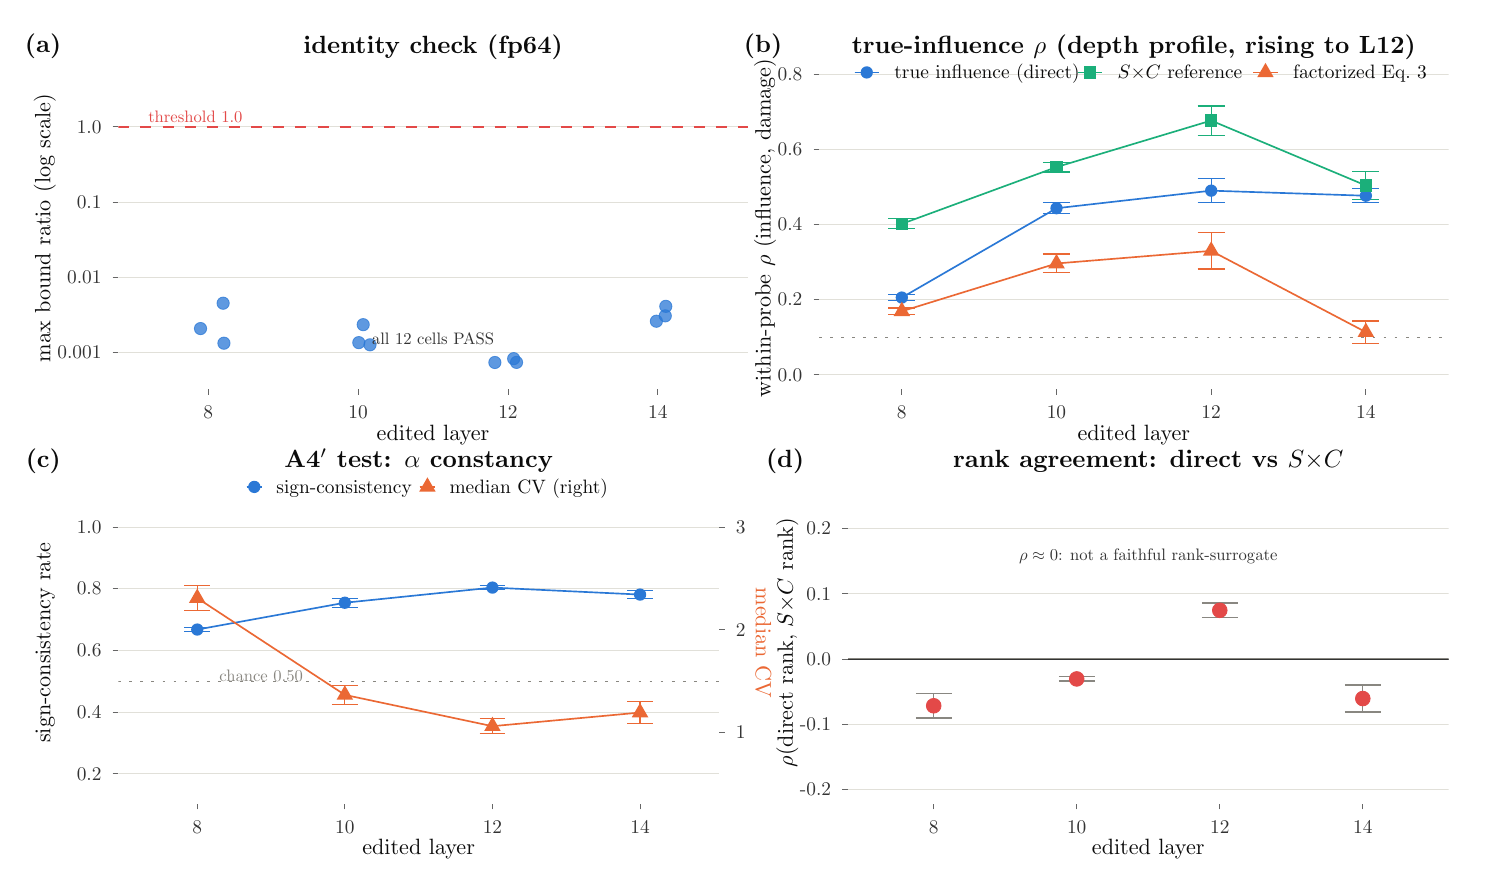
\begin{tikzpicture}[x=1pt,y=1pt]
\definecolor{fillColor}{RGB}{255,255,255}
\path[use as bounding box,fill=fillColor,fill opacity=0.00] (0,0) rectangle (517.45,303.53);
\begin{scope}
\path[clip] (  0.00,  0.00) rectangle (517.45,303.53);
\definecolor{drawColor}{RGB}{255,255,255}
\definecolor{fillColor}{RGB}{255,255,255}

\path[draw=drawColor,line width= 0.6pt,line join=round,line cap=round,fill=fillColor] (  0.00,  0.00) rectangle (517.45,303.53);
\end{scope}
\begin{scope}
\path[clip] (  2.00,151.77) rectangle (262.23,301.53);
\definecolor{fillColor}{RGB}{255,255,255}

\path[fill=fillColor] (  2.00,151.77) rectangle (262.23,301.53);
\end{scope}
\begin{scope}
\path[clip] (262.23,151.77) rectangle (515.45,301.53);
\definecolor{fillColor}{RGB}{255,255,255}

\path[fill=fillColor] (262.23,151.77) rectangle (515.45,301.53);
\end{scope}
\begin{scope}
\path[clip] ( 32.74,172.83) rectangle (260.23,289.31);
\definecolor{drawColor}{RGB}{225,224,217}

\path[draw=drawColor,line width= 0.3pt,line join=round] ( 32.74,186.29) --
	(260.23,186.29);

\path[draw=drawColor,line width= 0.3pt,line join=round] ( 32.74,213.42) --
	(260.23,213.42);

\path[draw=drawColor,line width= 0.3pt,line join=round] ( 32.74,240.55) --
	(260.23,240.55);

\path[draw=drawColor,line width= 0.3pt,line join=round] ( 32.74,267.68) --
	(260.23,267.68);
\definecolor{drawColor}{RGB}{227,73,72}

\path[draw=drawColor,line width= 0.6pt,dash pattern=on 4pt off 4pt ,line join=round] ( 32.74,267.68) -- (260.23,267.68);
\definecolor{drawColor}{RGB}{42,120,214}
\definecolor{fillColor}{RGB}{42,120,214}

\path[draw=drawColor,draw opacity=0.75,line width= 0.3pt,line join=round,line cap=round,fill=fillColor,fill opacity=0.75] ( 70.63,203.96) circle (  2.22);

\path[draw=drawColor,draw opacity=0.75,line width= 0.3pt,line join=round,line cap=round,fill=fillColor,fill opacity=0.75] ( 70.92,189.51) circle (  2.22);

\path[draw=drawColor,draw opacity=0.75,line width= 0.3pt,line join=round,line cap=round,fill=fillColor,fill opacity=0.75] ( 62.46,194.80) circle (  2.22);

\path[draw=drawColor,draw opacity=0.75,line width= 0.3pt,line join=round,line cap=round,fill=fillColor,fill opacity=0.75] (123.70,188.93) circle (  2.22);

\path[draw=drawColor,draw opacity=0.75,line width= 0.3pt,line join=round,line cap=round,fill=fillColor,fill opacity=0.75] (121.24,196.21) circle (  2.22);

\path[draw=drawColor,draw opacity=0.75,line width= 0.3pt,line join=round,line cap=round,fill=fillColor,fill opacity=0.75] (119.65,189.72) circle (  2.22);

\path[draw=drawColor,draw opacity=0.75,line width= 0.3pt,line join=round,line cap=round,fill=fillColor,fill opacity=0.75] (176.64,182.58) circle (  2.22);

\path[draw=drawColor,draw opacity=0.75,line width= 0.3pt,line join=round,line cap=round,fill=fillColor,fill opacity=0.75] (168.82,182.54) circle (  2.22);

\path[draw=drawColor,draw opacity=0.75,line width= 0.3pt,line join=round,line cap=round,fill=fillColor,fill opacity=0.75] (175.61,183.93) circle (  2.22);

\path[draw=drawColor,draw opacity=0.75,line width= 0.3pt,line join=round,line cap=round,fill=fillColor,fill opacity=0.75] (230.39,199.39) circle (  2.22);

\path[draw=drawColor,draw opacity=0.75,line width= 0.3pt,line join=round,line cap=round,fill=fillColor,fill opacity=0.75] (227.18,197.45) circle (  2.22);

\path[draw=drawColor,draw opacity=0.75,line width= 0.3pt,line join=round,line cap=round,fill=fillColor,fill opacity=0.75] (230.58,202.83) circle (  2.22);
\definecolor{drawColor}{RGB}{227,73,72}

\node[text=drawColor,anchor=base west,inner sep=0pt, outer sep=0pt, scale=  0.60] at ( 43.57,269.27) {threshold 1.0};
\definecolor{drawColor}{gray}{0.20}

\node[text=drawColor,anchor=base,inner sep=0pt, outer sep=0pt, scale=  0.60] at (146.48,189.12) {all 12 cells PASS};
\end{scope}
\begin{scope}
\path[clip] (  0.00,  0.00) rectangle (517.45,303.53);
\definecolor{drawColor}{gray}{0.20}

\node[text=drawColor,anchor=base east,inner sep=0pt, outer sep=0pt, scale=  0.70] at ( 26.69,184.01) {0.001};

\node[text=drawColor,anchor=base east,inner sep=0pt, outer sep=0pt, scale=  0.70] at ( 26.69,211.14) {0.01};

\node[text=drawColor,anchor=base east,inner sep=0pt, outer sep=0pt, scale=  0.70] at ( 26.69,238.27) {0.1};

\node[text=drawColor,anchor=base east,inner sep=0pt, outer sep=0pt, scale=  0.70] at ( 26.69,265.40) {1.0};
\end{scope}
\begin{scope}
\path[clip] (  0.00,  0.00) rectangle (517.45,303.53);
\definecolor{drawColor}{gray}{0.40}

\path[draw=drawColor,line width= 0.3pt,line join=round] ( 30.74,186.29) --
	( 32.74,186.29);

\path[draw=drawColor,line width= 0.3pt,line join=round] ( 30.74,213.42) --
	( 32.74,213.42);

\path[draw=drawColor,line width= 0.3pt,line join=round] ( 30.74,240.55) --
	( 32.74,240.55);

\path[draw=drawColor,line width= 0.3pt,line join=round] ( 30.74,267.68) --
	( 32.74,267.68);
\end{scope}
\begin{scope}
\path[clip] (  0.00,  0.00) rectangle (517.45,303.53);
\definecolor{drawColor}{gray}{0.40}

\path[draw=drawColor,line width= 0.3pt,line join=round] ( 65.24,170.83) --
	( 65.24,172.83);

\path[draw=drawColor,line width= 0.3pt,line join=round] (119.40,170.83) --
	(119.40,172.83);

\path[draw=drawColor,line width= 0.3pt,line join=round] (173.56,170.83) --
	(173.56,172.83);

\path[draw=drawColor,line width= 0.3pt,line join=round] (227.73,170.83) --
	(227.73,172.83);
\end{scope}
\begin{scope}
\path[clip] (  0.00,  0.00) rectangle (517.45,303.53);
\definecolor{drawColor}{gray}{0.20}

\node[text=drawColor,anchor=base,inner sep=0pt, outer sep=0pt, scale=  0.70] at ( 65.24,162.22) {8};

\node[text=drawColor,anchor=base,inner sep=0pt, outer sep=0pt, scale=  0.70] at (119.40,162.22) {10};

\node[text=drawColor,anchor=base,inner sep=0pt, outer sep=0pt, scale=  0.70] at (173.56,162.22) {12};

\node[text=drawColor,anchor=base,inner sep=0pt, outer sep=0pt, scale=  0.70] at (227.73,162.22) {14};
\end{scope}
\begin{scope}
\path[clip] (  0.00,  0.00) rectangle (517.45,303.53);
\definecolor{drawColor}{RGB}{11,11,11}

\node[text=drawColor,anchor=base,inner sep=0pt, outer sep=0pt, scale=  0.80] at (146.48,154.50) {edited layer};
\end{scope}
\begin{scope}
\path[clip] (  0.00,  0.00) rectangle (517.45,303.53);
\definecolor{drawColor}{RGB}{11,11,11}

\node[text=drawColor,rotate= 90.00,anchor=base,inner sep=0pt, outer sep=0pt, scale=  0.80] at (  8.21,231.07) {max bound ratio (log scale)};
\end{scope}
\begin{scope}
\path[clip] (  0.00,  0.00) rectangle (517.45,303.53);
\definecolor{drawColor}{RGB}{11,11,11}

\node[text=drawColor,anchor=base,inner sep=0pt, outer sep=0pt, scale=  0.90] at (146.48,294.33) {\bfseries identity check (fp64)};
\end{scope}
\begin{scope}
\path[clip] (  0.00,  0.00) rectangle (517.45,303.53);
\definecolor{drawColor}{RGB}{11,11,11}

\node[text=drawColor,anchor=base,inner sep=0pt, outer sep=0pt, scale=  0.90] at (  5.57,294.48) {\bfseries (a)};
\end{scope}
\begin{scope}
\path[clip] (285.97,172.83) rectangle (513.45,289.31);
\definecolor{drawColor}{RGB}{225,224,217}

\path[draw=drawColor,line width= 0.3pt,line join=round] (285.97,178.12) --
	(513.45,178.12);

\path[draw=drawColor,line width= 0.3pt,line join=round] (285.97,205.28) --
	(513.45,205.28);

\path[draw=drawColor,line width= 0.3pt,line join=round] (285.97,232.43) --
	(513.45,232.43);

\path[draw=drawColor,line width= 0.3pt,line join=round] (285.97,259.58) --
	(513.45,259.58);

\path[draw=drawColor,line width= 0.3pt,line join=round] (285.97,286.73) --
	(513.45,286.73);
\definecolor{drawColor}{RGB}{137,135,129}

\path[draw=drawColor,line width= 0.3pt,dash pattern=on 1pt off 3pt ,line join=round] (285.97,191.70) -- (513.45,191.70);
\definecolor{drawColor}{RGB}{42,120,214}

\path[draw=drawColor,line width= 0.4pt,line join=round] (310.98,207.13) --
	(320.76,207.13);

\path[draw=drawColor,line width= 0.4pt,line join=round] (315.87,207.13) --
	(315.87,204.87);

\path[draw=drawColor,line width= 0.4pt,line join=round] (310.98,204.87) --
	(320.76,204.87);

\path[draw=drawColor,line width= 0.4pt,line join=round] (366.87,240.26) --
	(376.65,240.26);

\path[draw=drawColor,line width= 0.4pt,line join=round] (371.76,240.26) --
	(371.76,236.31);

\path[draw=drawColor,line width= 0.4pt,line join=round] (366.87,236.31) --
	(376.65,236.31);

\path[draw=drawColor,line width= 0.4pt,line join=round] (422.77,248.87) --
	(432.55,248.87);

\path[draw=drawColor,line width= 0.4pt,line join=round] (427.66,248.87) --
	(427.66,240.38);

\path[draw=drawColor,line width= 0.4pt,line join=round] (422.77,240.38) --
	(432.55,240.38);

\path[draw=drawColor,line width= 0.4pt,line join=round] (478.66,245.34) --
	(488.44,245.34);

\path[draw=drawColor,line width= 0.4pt,line join=round] (483.55,245.34) --
	(483.55,240.26);

\path[draw=drawColor,line width= 0.4pt,line join=round] (478.66,240.26) --
	(488.44,240.26);
\definecolor{drawColor}{RGB}{27,175,122}

\path[draw=drawColor,line width= 0.4pt,line join=round] (310.98,234.45) --
	(320.76,234.45);

\path[draw=drawColor,line width= 0.4pt,line join=round] (315.87,234.45) --
	(315.87,230.81);

\path[draw=drawColor,line width= 0.4pt,line join=round] (310.98,230.81) --
	(320.76,230.81);

\path[draw=drawColor,line width= 0.4pt,line join=round] (366.87,254.92) --
	(376.65,254.92);

\path[draw=drawColor,line width= 0.4pt,line join=round] (371.76,254.92) --
	(371.76,251.37);

\path[draw=drawColor,line width= 0.4pt,line join=round] (366.87,251.37) --
	(376.65,251.37);

\path[draw=drawColor,line width= 0.4pt,line join=round] (422.77,275.23) --
	(432.55,275.23);

\path[draw=drawColor,line width= 0.4pt,line join=round] (427.66,275.23) --
	(427.66,264.69);

\path[draw=drawColor,line width= 0.4pt,line join=round] (422.77,264.69) --
	(432.55,264.69);

\path[draw=drawColor,line width= 0.4pt,line join=round] (478.66,251.44) --
	(488.44,251.44);

\path[draw=drawColor,line width= 0.4pt,line join=round] (483.55,251.44) --
	(483.55,241.55);

\path[draw=drawColor,line width= 0.4pt,line join=round] (478.66,241.55) --
	(488.44,241.55);
\definecolor{drawColor}{RGB}{235,104,52}

\path[draw=drawColor,line width= 0.4pt,line join=round] (310.98,202.24) --
	(320.76,202.24);

\path[draw=drawColor,line width= 0.4pt,line join=round] (315.87,202.24) --
	(315.87,199.83);

\path[draw=drawColor,line width= 0.4pt,line join=round] (310.98,199.83) --
	(320.76,199.83);

\path[draw=drawColor,line width= 0.4pt,line join=round] (366.87,221.73) --
	(376.65,221.73);

\path[draw=drawColor,line width= 0.4pt,line join=round] (371.76,221.73) --
	(371.76,214.91);

\path[draw=drawColor,line width= 0.4pt,line join=round] (366.87,214.91) --
	(376.65,214.91);

\path[draw=drawColor,line width= 0.4pt,line join=round] (422.77,229.44) --
	(432.55,229.44);

\path[draw=drawColor,line width= 0.4pt,line join=round] (427.66,229.44) --
	(427.66,216.33);

\path[draw=drawColor,line width= 0.4pt,line join=round] (422.77,216.33) --
	(432.55,216.33);

\path[draw=drawColor,line width= 0.4pt,line join=round] (478.66,197.52) --
	(488.44,197.52);

\path[draw=drawColor,line width= 0.4pt,line join=round] (483.55,197.52) --
	(483.55,189.51);

\path[draw=drawColor,line width= 0.4pt,line join=round] (478.66,189.51) --
	(488.44,189.51);
\definecolor{drawColor}{RGB}{42,120,214}

\path[draw=drawColor,line width= 0.6pt,line join=round] (315.87,206.00) --
	(371.76,238.28) --
	(427.66,244.63) --
	(483.55,242.80);
\definecolor{drawColor}{RGB}{27,175,122}

\path[draw=drawColor,line width= 0.6pt,line join=round] (315.87,232.63) --
	(371.76,253.15) --
	(427.66,269.96) --
	(483.55,246.50);
\definecolor{drawColor}{RGB}{235,104,52}

\path[draw=drawColor,line width= 0.6pt,line join=round] (315.87,201.04) --
	(371.76,218.32) --
	(427.66,222.88) --
	(483.55,193.51);
\definecolor{fillColor}{RGB}{42,120,214}

\path[fill=fillColor] (315.87,206.00) circle (  2.22);

\path[fill=fillColor] (371.76,238.28) circle (  2.22);

\path[fill=fillColor] (427.66,244.63) circle (  2.22);

\path[fill=fillColor] (483.55,242.80) circle (  2.22);
\definecolor{fillColor}{RGB}{27,175,122}

\path[fill=fillColor] (313.65,230.41) --
	(318.09,230.41) --
	(318.09,234.85) --
	(313.65,234.85) --
	cycle;

\path[fill=fillColor] (369.54,250.93) --
	(373.98,250.93) --
	(373.98,255.36) --
	(369.54,255.36) --
	cycle;

\path[fill=fillColor] (425.44,267.74) --
	(429.88,267.74) --
	(429.88,272.18) --
	(425.44,272.18) --
	cycle;

\path[fill=fillColor] (481.33,244.28) --
	(485.77,244.28) --
	(485.77,248.72) --
	(481.33,248.72) --
	cycle;
\definecolor{fillColor}{RGB}{235,104,52}

\path[fill=fillColor] (315.87,204.49) --
	(318.86,199.31) --
	(312.88,199.31) --
	cycle;

\path[fill=fillColor] (371.76,221.77) --
	(374.75,216.59) --
	(368.77,216.59) --
	cycle;

\path[fill=fillColor] (427.66,226.33) --
	(430.64,221.16) --
	(424.67,221.16) --
	cycle;

\path[fill=fillColor] (483.55,196.97) --
	(486.54,191.79) --
	(480.56,191.79) --
	cycle;
\end{scope}
\begin{scope}
\path[clip] (  0.00,  0.00) rectangle (517.45,303.53);
\definecolor{drawColor}{gray}{0.20}

\node[text=drawColor,anchor=base east,inner sep=0pt, outer sep=0pt, scale=  0.70] at (279.92,175.85) {0.0};

\node[text=drawColor,anchor=base east,inner sep=0pt, outer sep=0pt, scale=  0.70] at (279.92,203.00) {0.2};

\node[text=drawColor,anchor=base east,inner sep=0pt, outer sep=0pt, scale=  0.70] at (279.92,230.15) {0.4};

\node[text=drawColor,anchor=base east,inner sep=0pt, outer sep=0pt, scale=  0.70] at (279.92,257.30) {0.6};

\node[text=drawColor,anchor=base east,inner sep=0pt, outer sep=0pt, scale=  0.70] at (279.92,284.45) {0.8};
\end{scope}
\begin{scope}
\path[clip] (  0.00,  0.00) rectangle (517.45,303.53);
\definecolor{drawColor}{gray}{0.40}

\path[draw=drawColor,line width= 0.3pt,line join=round] (283.97,178.12) --
	(285.97,178.12);

\path[draw=drawColor,line width= 0.3pt,line join=round] (283.97,205.28) --
	(285.97,205.28);

\path[draw=drawColor,line width= 0.3pt,line join=round] (283.97,232.43) --
	(285.97,232.43);

\path[draw=drawColor,line width= 0.3pt,line join=round] (283.97,259.58) --
	(285.97,259.58);

\path[draw=drawColor,line width= 0.3pt,line join=round] (283.97,286.73) --
	(285.97,286.73);
\end{scope}
\begin{scope}
\path[clip] (  0.00,  0.00) rectangle (517.45,303.53);
\definecolor{drawColor}{gray}{0.40}

\path[draw=drawColor,line width= 0.3pt,line join=round] (315.87,170.83) --
	(315.87,172.83);

\path[draw=drawColor,line width= 0.3pt,line join=round] (371.76,170.83) --
	(371.76,172.83);

\path[draw=drawColor,line width= 0.3pt,line join=round] (427.66,170.83) --
	(427.66,172.83);

\path[draw=drawColor,line width= 0.3pt,line join=round] (483.55,170.83) --
	(483.55,172.83);
\end{scope}
\begin{scope}
\path[clip] (  0.00,  0.00) rectangle (517.45,303.53);
\definecolor{drawColor}{gray}{0.20}

\node[text=drawColor,anchor=base,inner sep=0pt, outer sep=0pt, scale=  0.70] at (315.87,162.22) {8};

\node[text=drawColor,anchor=base,inner sep=0pt, outer sep=0pt, scale=  0.70] at (371.76,162.22) {10};

\node[text=drawColor,anchor=base,inner sep=0pt, outer sep=0pt, scale=  0.70] at (427.66,162.22) {12};

\node[text=drawColor,anchor=base,inner sep=0pt, outer sep=0pt, scale=  0.70] at (483.55,162.22) {14};
\end{scope}
\begin{scope}
\path[clip] (  0.00,  0.00) rectangle (517.45,303.53);
\definecolor{drawColor}{RGB}{11,11,11}

\node[text=drawColor,anchor=base,inner sep=0pt, outer sep=0pt, scale=  0.80] at (399.71,154.50) {edited layer};
\end{scope}
\begin{scope}
\path[clip] (  0.00,  0.00) rectangle (517.45,303.53);
\definecolor{drawColor}{RGB}{11,11,11}

\node[text=drawColor,rotate= 90.00,anchor=base,inner sep=0pt, outer sep=0pt, scale=  0.80] at (268.43,231.07) {within-probe $\rho$ (influence, damage)};
\end{scope}
\begin{scope}
\path[clip] (  0.00,  0.00) rectangle (517.45,303.53);
\definecolor{drawColor}{RGB}{42,120,214}

\path[draw=drawColor,line width= 0.4pt,line join=round] (298.80,287.35) -- (307.60,287.35);

\path[draw=drawColor,line width= 0.6pt,line join=round] (298.80,287.35) -- (307.60,287.35);
\definecolor{fillColor}{RGB}{42,120,214}

\path[fill=fillColor] (303.20,287.35) circle (  2.22);
\end{scope}
\begin{scope}
\path[clip] (  0.00,  0.00) rectangle (517.45,303.53);
\definecolor{drawColor}{RGB}{27,175,122}

\path[draw=drawColor,line width= 0.4pt,line join=round] (379.45,287.35) -- (388.25,287.35);

\path[draw=drawColor,line width= 0.6pt,line join=round] (379.45,287.35) -- (388.25,287.35);
\definecolor{fillColor}{RGB}{27,175,122}

\path[fill=fillColor] (381.63,285.13) --
	(386.07,285.13) --
	(386.07,289.57) --
	(381.63,289.57) --
	cycle;
\end{scope}
\begin{scope}
\path[clip] (  0.00,  0.00) rectangle (517.45,303.53);
\definecolor{drawColor}{RGB}{235,104,52}

\path[draw=drawColor,line width= 0.4pt,line join=round] (442.88,287.35) -- (451.68,287.35);

\path[draw=drawColor,line width= 0.6pt,line join=round] (442.88,287.35) -- (451.68,287.35);
\definecolor{fillColor}{RGB}{235,104,52}

\path[fill=fillColor] (447.28,290.80) --
	(450.26,285.62) --
	(444.29,285.62) --
	cycle;
\end{scope}
\begin{scope}
\path[clip] (  0.00,  0.00) rectangle (517.45,303.53);
\definecolor{drawColor}{RGB}{11,11,11}

\node[text=drawColor,anchor=base west,inner sep=0pt, outer sep=0pt, scale=  0.70] at (313.20,285.07) {true influence (direct)};
\end{scope}
\begin{scope}
\path[clip] (  0.00,  0.00) rectangle (517.45,303.53);
\definecolor{drawColor}{RGB}{11,11,11}

\node[text=drawColor,anchor=base west,inner sep=0pt, outer sep=0pt, scale=  0.70] at (393.85,285.07) {$S{\times}C$ reference};
\end{scope}
\begin{scope}
\path[clip] (  0.00,  0.00) rectangle (517.45,303.53);
\definecolor{drawColor}{RGB}{11,11,11}

\node[text=drawColor,anchor=base west,inner sep=0pt, outer sep=0pt, scale=  0.70] at (457.28,285.07) {factorized Eq.~3};
\end{scope}
\begin{scope}
\path[clip] (  0.00,  0.00) rectangle (517.45,303.53);
\definecolor{drawColor}{RGB}{11,11,11}

\node[text=drawColor,anchor=base,inner sep=0pt, outer sep=0pt, scale=  0.90] at (399.71,294.33) {\bfseries true-influence $\rho$ (depth profile, rising to L12)};
\end{scope}
\begin{scope}
\path[clip] (  0.00,  0.00) rectangle (517.45,303.53);
\definecolor{drawColor}{RGB}{11,11,11}

\node[text=drawColor,anchor=base,inner sep=0pt, outer sep=0pt, scale=  0.90] at (265.73,294.48) {\bfseries (b)};
\end{scope}
\begin{scope}
\path[clip] (  2.00,  2.00) rectangle (270.31,151.77);
\definecolor{fillColor}{RGB}{255,255,255}

\path[fill=fillColor] (  2.00,  2.00) rectangle (270.31,151.77);
\end{scope}
\begin{scope}
\path[clip] (270.31,  2.00) rectangle (515.45,151.77);
\definecolor{fillColor}{RGB}{255,255,255}

\path[fill=fillColor] (270.31,  2.00) rectangle (515.45,151.77);
\end{scope}
\begin{scope}
\path[clip] ( 32.74, 23.06) rectangle (249.82,139.55);
\definecolor{drawColor}{RGB}{225,224,217}

\path[draw=drawColor,line width= 0.3pt,line join=round] ( 32.74, 33.93) --
	(249.82, 33.93);

\path[draw=drawColor,line width= 0.3pt,line join=round] ( 32.74, 56.22) --
	(249.82, 56.22);

\path[draw=drawColor,line width= 0.3pt,line join=round] ( 32.74, 78.52) --
	(249.82, 78.52);

\path[draw=drawColor,line width= 0.3pt,line join=round] ( 32.74,100.81) --
	(249.82,100.81);

\path[draw=drawColor,line width= 0.3pt,line join=round] ( 32.74,123.10) --
	(249.82,123.10);
\definecolor{drawColor}{RGB}{137,135,129}

\path[draw=drawColor,line width= 0.5pt,dash pattern=on 1pt off 3pt ,line join=round] ( 32.74, 67.37) -- (249.82, 67.37);

\node[text=drawColor,anchor=base west,inner sep=0pt, outer sep=0pt, scale=  0.60] at ( 69.27, 67.10) {chance 0.50};
\definecolor{drawColor}{RGB}{42,120,214}

\path[draw=drawColor,line width= 0.4pt,line join=round] ( 56.61, 86.65) --
	( 65.94, 86.65);

\path[draw=drawColor,line width= 0.4pt,line join=round] ( 61.27, 86.65) --
	( 61.27, 85.43);

\path[draw=drawColor,line width= 0.4pt,line join=round] ( 56.61, 85.43) --
	( 65.94, 85.43);

\path[draw=drawColor,line width= 0.4pt,line join=round] (109.94, 97.30) --
	(119.28, 97.30);

\path[draw=drawColor,line width= 0.4pt,line join=round] (114.61, 97.30) --
	(114.61, 94.15);

\path[draw=drawColor,line width= 0.4pt,line join=round] (109.94, 94.15) --
	(119.28, 94.15);

\path[draw=drawColor,line width= 0.4pt,line join=round] (163.28,102.03) --
	(172.61,102.03);

\path[draw=drawColor,line width= 0.4pt,line join=round] (167.95,102.03) --
	(167.95,100.38);

\path[draw=drawColor,line width= 0.4pt,line join=round] (163.28,100.38) --
	(172.61,100.38);

\path[draw=drawColor,line width= 0.4pt,line join=round] (216.61,100.16) --
	(225.95,100.16);

\path[draw=drawColor,line width= 0.4pt,line join=round] (221.28,100.16) --
	(221.28, 97.20);

\path[draw=drawColor,line width= 0.4pt,line join=round] (216.61, 97.20) --
	(225.95, 97.20);
\definecolor{drawColor}{RGB}{235,104,52}

\path[draw=drawColor,line width= 0.4pt,line join=round] ( 56.61,102.00) --
	( 65.94,102.00);

\path[draw=drawColor,line width= 0.4pt,line join=round] ( 61.27,102.00) --
	( 61.27, 92.81);

\path[draw=drawColor,line width= 0.4pt,line join=round] ( 56.61, 92.81) --
	( 65.94, 92.81);

\path[draw=drawColor,line width= 0.4pt,line join=round] (109.94, 65.81) --
	(119.28, 65.81);

\path[draw=drawColor,line width= 0.4pt,line join=round] (114.61, 65.81) --
	(114.61, 59.04);

\path[draw=drawColor,line width= 0.4pt,line join=round] (109.94, 59.04) --
	(119.28, 59.04);

\path[draw=drawColor,line width= 0.4pt,line join=round] (163.28, 53.76) --
	(172.61, 53.76);

\path[draw=drawColor,line width= 0.4pt,line join=round] (167.95, 53.76) --
	(167.95, 48.48);

\path[draw=drawColor,line width= 0.4pt,line join=round] (163.28, 48.48) --
	(172.61, 48.48);

\path[draw=drawColor,line width= 0.4pt,line join=round] (216.61, 60.00) --
	(225.95, 60.00);

\path[draw=drawColor,line width= 0.4pt,line join=round] (221.28, 60.00) --
	(221.28, 52.10);

\path[draw=drawColor,line width= 0.4pt,line join=round] (216.61, 52.10) --
	(225.95, 52.10);
\definecolor{drawColor}{RGB}{42,120,214}

\path[draw=drawColor,line width= 0.6pt,line join=round] ( 61.27, 86.04) --
	(114.61, 95.73) --
	(167.95,101.20) --
	(221.28, 98.68);
\definecolor{drawColor}{RGB}{235,104,52}

\path[draw=drawColor,line width= 0.6pt,line join=round] ( 61.27, 97.41) --
	(114.61, 62.43) --
	(167.95, 51.12) --
	(221.28, 56.05);
\definecolor{fillColor}{RGB}{42,120,214}

\path[fill=fillColor] ( 61.27, 86.04) circle (  2.22);

\path[fill=fillColor] (114.61, 95.73) circle (  2.22);

\path[fill=fillColor] (167.95,101.20) circle (  2.22);

\path[fill=fillColor] (221.28, 98.68) circle (  2.22);
\definecolor{fillColor}{RGB}{235,104,52}

\path[fill=fillColor] ( 61.27,100.86) --
	( 64.26, 95.68) --
	( 58.29, 95.68) --
	cycle;

\path[fill=fillColor] (114.61, 65.88) --
	(117.60, 60.70) --
	(111.62, 60.70) --
	cycle;

\path[fill=fillColor] (167.95, 54.57) --
	(170.93, 49.39) --
	(164.96, 49.39) --
	cycle;

\path[fill=fillColor] (221.28, 59.50) --
	(224.27, 54.33) --
	(218.29, 54.33) --
	cycle;
\end{scope}
\begin{scope}
\path[clip] (  0.00,  0.00) rectangle (517.45,303.53);
\definecolor{drawColor}{gray}{0.20}

\node[text=drawColor,anchor=base east,inner sep=0pt, outer sep=0pt, scale=  0.70] at ( 26.69, 31.65) {0.2};

\node[text=drawColor,anchor=base east,inner sep=0pt, outer sep=0pt, scale=  0.70] at ( 26.69, 53.95) {0.4};

\node[text=drawColor,anchor=base east,inner sep=0pt, outer sep=0pt, scale=  0.70] at ( 26.69, 76.24) {0.6};

\node[text=drawColor,anchor=base east,inner sep=0pt, outer sep=0pt, scale=  0.70] at ( 26.69, 98.53) {0.8};

\node[text=drawColor,anchor=base east,inner sep=0pt, outer sep=0pt, scale=  0.70] at ( 26.69,120.83) {1.0};
\end{scope}
\begin{scope}
\path[clip] (  0.00,  0.00) rectangle (517.45,303.53);
\definecolor{drawColor}{gray}{0.40}

\path[draw=drawColor,line width= 0.3pt,line join=round] ( 30.74, 33.93) --
	( 32.74, 33.93);

\path[draw=drawColor,line width= 0.3pt,line join=round] ( 30.74, 56.22) --
	( 32.74, 56.22);

\path[draw=drawColor,line width= 0.3pt,line join=round] ( 30.74, 78.52) --
	( 32.74, 78.52);

\path[draw=drawColor,line width= 0.3pt,line join=round] ( 30.74,100.81) --
	( 32.74,100.81);

\path[draw=drawColor,line width= 0.3pt,line join=round] ( 30.74,123.10) --
	( 32.74,123.10);
\end{scope}
\begin{scope}
\path[clip] (  0.00,  0.00) rectangle (517.45,303.53);
\definecolor{drawColor}{gray}{0.40}

\path[draw=drawColor,line width= 0.3pt,line join=round] (251.82, 48.79) --
	(249.82, 48.79);

\path[draw=drawColor,line width= 0.3pt,line join=round] (251.82, 85.95) --
	(249.82, 85.95);

\path[draw=drawColor,line width= 0.3pt,line join=round] (251.82,123.10) --
	(249.82,123.10);
\end{scope}
\begin{scope}
\path[clip] (  0.00,  0.00) rectangle (517.45,303.53);
\definecolor{drawColor}{gray}{0.20}

\node[text=drawColor,anchor=base east,inner sep=0pt, outer sep=0pt, scale=  0.70] at (259.37, 46.51) {1};

\node[text=drawColor,anchor=base east,inner sep=0pt, outer sep=0pt, scale=  0.70] at (259.37, 83.67) {2};

\node[text=drawColor,anchor=base east,inner sep=0pt, outer sep=0pt, scale=  0.70] at (259.37,120.83) {3};
\end{scope}
\begin{scope}
\path[clip] (  0.00,  0.00) rectangle (517.45,303.53);
\definecolor{drawColor}{gray}{0.40}

\path[draw=drawColor,line width= 0.3pt,line join=round] ( 61.27, 21.06) --
	( 61.27, 23.06);

\path[draw=drawColor,line width= 0.3pt,line join=round] (114.61, 21.06) --
	(114.61, 23.06);

\path[draw=drawColor,line width= 0.3pt,line join=round] (167.95, 21.06) --
	(167.95, 23.06);

\path[draw=drawColor,line width= 0.3pt,line join=round] (221.28, 21.06) --
	(221.28, 23.06);
\end{scope}
\begin{scope}
\path[clip] (  0.00,  0.00) rectangle (517.45,303.53);
\definecolor{drawColor}{gray}{0.20}

\node[text=drawColor,anchor=base,inner sep=0pt, outer sep=0pt, scale=  0.70] at ( 61.27, 12.46) {8};

\node[text=drawColor,anchor=base,inner sep=0pt, outer sep=0pt, scale=  0.70] at (114.61, 12.46) {10};

\node[text=drawColor,anchor=base,inner sep=0pt, outer sep=0pt, scale=  0.70] at (167.95, 12.46) {12};

\node[text=drawColor,anchor=base,inner sep=0pt, outer sep=0pt, scale=  0.70] at (221.28, 12.46) {14};
\end{scope}
\begin{scope}
\path[clip] (  0.00,  0.00) rectangle (517.45,303.53);
\definecolor{drawColor}{RGB}{11,11,11}

\node[text=drawColor,anchor=base,inner sep=0pt, outer sep=0pt, scale=  0.80] at (141.28,  4.73) {edited layer};
\end{scope}
\begin{scope}
\path[clip] (  0.00,  0.00) rectangle (517.45,303.53);
\definecolor{drawColor}{RGB}{11,11,11}

\node[text=drawColor,rotate= 90.00,anchor=base,inner sep=0pt, outer sep=0pt, scale=  0.80] at (  8.21, 81.30) {sign-consistency rate};
\end{scope}
\begin{scope}
\path[clip] (  0.00,  0.00) rectangle (517.45,303.53);
\definecolor{drawColor}{RGB}{235,104,52}

\node[text=drawColor,rotate=-90.00,anchor=base,inner sep=0pt, outer sep=0pt, scale=  0.80] at (263.10, 81.30) {median CV};
\end{scope}
\begin{scope}
\path[clip] (  0.00,  0.00) rectangle (517.45,303.53);
\definecolor{drawColor}{RGB}{42,120,214}

\path[draw=drawColor,line width= 0.4pt,line join=round] ( 79.09,137.58) -- ( 84.69,137.58);

\path[draw=drawColor,line width= 0.6pt,line join=round] ( 79.09,137.58) -- ( 84.69,137.58);
\definecolor{fillColor}{RGB}{42,120,214}

\path[fill=fillColor] ( 81.89,137.58) circle (  2.22);
\end{scope}
\begin{scope}
\path[clip] (  0.00,  0.00) rectangle (517.45,303.53);
\definecolor{drawColor}{RGB}{235,104,52}

\path[draw=drawColor,line width= 0.4pt,line join=round] (141.65,137.58) -- (147.25,137.58);

\path[draw=drawColor,line width= 0.6pt,line join=round] (141.65,137.58) -- (147.25,137.58);
\definecolor{fillColor}{RGB}{235,104,52}

\path[fill=fillColor] (144.45,141.03) --
	(147.44,135.86) --
	(141.46,135.86) --
	cycle;
\end{scope}
\begin{scope}
\path[clip] (  0.00,  0.00) rectangle (517.45,303.53);
\definecolor{drawColor}{RGB}{11,11,11}

\node[text=drawColor,anchor=base west,inner sep=0pt, outer sep=0pt, scale=  0.70] at ( 89.89,135.30) {sign-consistency};
\end{scope}
\begin{scope}
\path[clip] (  0.00,  0.00) rectangle (517.45,303.53);
\definecolor{drawColor}{RGB}{11,11,11}

\node[text=drawColor,anchor=base west,inner sep=0pt, outer sep=0pt, scale=  0.70] at (152.45,135.30) {median CV (right)};
\end{scope}
\begin{scope}
\path[clip] (  0.00,  0.00) rectangle (517.45,303.53);
\definecolor{drawColor}{RGB}{11,11,11}

\node[text=drawColor,anchor=base,inner sep=0pt, outer sep=0pt, scale=  0.90] at (141.28,144.57) {\bfseries A4$'$ test: $\alpha$ constancy};
\end{scope}
\begin{scope}
\path[clip] (  0.00,  0.00) rectangle (517.45,303.53);
\definecolor{drawColor}{RGB}{11,11,11}

\node[text=drawColor,anchor=base,inner sep=0pt, outer sep=0pt, scale=  0.90] at (  5.65,144.71) {\bfseries (c)};
\end{scope}
\begin{scope}
\path[clip] (296.38, 23.06) rectangle (513.45,139.55);
\definecolor{drawColor}{RGB}{225,224,217}

\path[draw=drawColor,line width= 0.3pt,line join=round] (296.38, 28.36) --
	(513.45, 28.36);

\path[draw=drawColor,line width= 0.3pt,line join=round] (296.38, 51.89) --
	(513.45, 51.89);

\path[draw=drawColor,line width= 0.3pt,line join=round] (296.38, 75.42) --
	(513.45, 75.42);

\path[draw=drawColor,line width= 0.3pt,line join=round] (296.38, 98.95) --
	(513.45, 98.95);

\path[draw=drawColor,line width= 0.3pt,line join=round] (296.38,122.48) --
	(513.45,122.48);
\definecolor{drawColor}{RGB}{137,135,129}

\path[draw=drawColor,line width= 0.5pt,line join=round] (296.38, 75.42) -- (513.45, 75.42);

\path[draw=drawColor,line width= 0.5pt,line join=round] (320.93, 62.99) --
	(333.85, 62.99);

\path[draw=drawColor,line width= 0.5pt,line join=round] (327.39, 62.99) --
	(327.39, 54.02);

\path[draw=drawColor,line width= 0.5pt,line join=round] (320.93, 54.02) --
	(333.85, 54.02);

\path[draw=drawColor,line width= 0.5pt,line join=round] (372.61, 68.99) --
	(385.53, 68.99);

\path[draw=drawColor,line width= 0.5pt,line join=round] (379.07, 68.99) --
	(379.07, 67.40);

\path[draw=drawColor,line width= 0.5pt,line join=round] (372.61, 67.40) --
	(385.53, 67.40);

\path[draw=drawColor,line width= 0.5pt,line join=round] (424.30, 95.64) --
	(437.22, 95.64);

\path[draw=drawColor,line width= 0.5pt,line join=round] (430.76, 95.64) --
	(430.76, 90.34);

\path[draw=drawColor,line width= 0.5pt,line join=round] (424.30, 90.34) --
	(437.22, 90.34);

\path[draw=drawColor,line width= 0.5pt,line join=round] (475.98, 66.04) --
	(488.90, 66.04);

\path[draw=drawColor,line width= 0.5pt,line join=round] (482.44, 66.04) --
	(482.44, 56.19);

\path[draw=drawColor,line width= 0.5pt,line join=round] (475.98, 56.19) --
	(488.90, 56.19);
\definecolor{drawColor}{RGB}{227,73,72}
\definecolor{fillColor}{RGB}{227,73,72}

\path[draw=drawColor,line width= 0.3pt,line join=round,line cap=round,fill=fillColor] (327.39, 58.50) circle (  2.65);

\path[draw=drawColor,line width= 0.3pt,line join=round,line cap=round,fill=fillColor] (379.07, 68.20) circle (  2.65);

\path[draw=drawColor,line width= 0.3pt,line join=round,line cap=round,fill=fillColor] (430.76, 92.99) circle (  2.65);

\path[draw=drawColor,line width= 0.3pt,line join=round,line cap=round,fill=fillColor] (482.44, 61.11) circle (  2.65);
\definecolor{drawColor}{gray}{0.20}

\path[draw=drawColor,line width= 0.3pt,line join=round] (296.38, 75.42) -- (513.45, 75.42);

\node[text=drawColor,anchor=base,inner sep=0pt, outer sep=0pt, scale=  0.60] at (404.91,111.13) {$\rho \approx 0$: not a faithful rank-surrogate};
\end{scope}
\begin{scope}
\path[clip] (  0.00,  0.00) rectangle (517.45,303.53);
\definecolor{drawColor}{gray}{0.20}

\node[text=drawColor,anchor=base east,inner sep=0pt, outer sep=0pt, scale=  0.70] at (290.33, 26.08) {-0.2};

\node[text=drawColor,anchor=base east,inner sep=0pt, outer sep=0pt, scale=  0.70] at (290.33, 49.61) {-0.1};

\node[text=drawColor,anchor=base east,inner sep=0pt, outer sep=0pt, scale=  0.70] at (290.33, 73.14) {0.0};

\node[text=drawColor,anchor=base east,inner sep=0pt, outer sep=0pt, scale=  0.70] at (290.33, 96.67) {0.1};

\node[text=drawColor,anchor=base east,inner sep=0pt, outer sep=0pt, scale=  0.70] at (290.33,120.21) {0.2};
\end{scope}
\begin{scope}
\path[clip] (  0.00,  0.00) rectangle (517.45,303.53);
\definecolor{drawColor}{gray}{0.40}

\path[draw=drawColor,line width= 0.3pt,line join=round] (294.38, 28.36) --
	(296.38, 28.36);

\path[draw=drawColor,line width= 0.3pt,line join=round] (294.38, 51.89) --
	(296.38, 51.89);

\path[draw=drawColor,line width= 0.3pt,line join=round] (294.38, 75.42) --
	(296.38, 75.42);

\path[draw=drawColor,line width= 0.3pt,line join=round] (294.38, 98.95) --
	(296.38, 98.95);

\path[draw=drawColor,line width= 0.3pt,line join=round] (294.38,122.48) --
	(296.38,122.48);
\end{scope}
\begin{scope}
\path[clip] (  0.00,  0.00) rectangle (517.45,303.53);
\definecolor{drawColor}{gray}{0.40}

\path[draw=drawColor,line width= 0.3pt,line join=round] (327.39, 21.06) --
	(327.39, 23.06);

\path[draw=drawColor,line width= 0.3pt,line join=round] (379.07, 21.06) --
	(379.07, 23.06);

\path[draw=drawColor,line width= 0.3pt,line join=round] (430.76, 21.06) --
	(430.76, 23.06);

\path[draw=drawColor,line width= 0.3pt,line join=round] (482.44, 21.06) --
	(482.44, 23.06);
\end{scope}
\begin{scope}
\path[clip] (  0.00,  0.00) rectangle (517.45,303.53);
\definecolor{drawColor}{gray}{0.20}

\node[text=drawColor,anchor=base,inner sep=0pt, outer sep=0pt, scale=  0.70] at (327.39, 12.46) {8};

\node[text=drawColor,anchor=base,inner sep=0pt, outer sep=0pt, scale=  0.70] at (379.07, 12.46) {10};

\node[text=drawColor,anchor=base,inner sep=0pt, outer sep=0pt, scale=  0.70] at (430.76, 12.46) {12};

\node[text=drawColor,anchor=base,inner sep=0pt, outer sep=0pt, scale=  0.70] at (482.44, 12.46) {14};
\end{scope}
\begin{scope}
\path[clip] (  0.00,  0.00) rectangle (517.45,303.53);
\definecolor{drawColor}{RGB}{11,11,11}

\node[text=drawColor,anchor=base,inner sep=0pt, outer sep=0pt, scale=  0.80] at (404.91,  4.73) {edited layer};
\end{scope}
\begin{scope}
\path[clip] (  0.00,  0.00) rectangle (517.45,303.53);
\definecolor{drawColor}{RGB}{11,11,11}

\node[text=drawColor,rotate= 90.00,anchor=base,inner sep=0pt, outer sep=0pt, scale=  0.80] at (276.51, 81.30) {$\rho$(direct rank, $S{\times}C$ rank)};
\end{scope}
\begin{scope}
\path[clip] (  0.00,  0.00) rectangle (517.45,303.53);
\definecolor{drawColor}{RGB}{11,11,11}

\node[text=drawColor,anchor=base,inner sep=0pt, outer sep=0pt, scale=  0.90] at (404.91,144.57) {\bfseries rank agreement: direct vs $S{\times}C$};
\end{scope}
\begin{scope}
\path[clip] (  0.00,  0.00) rectangle (517.45,303.53);
\definecolor{drawColor}{RGB}{11,11,11}

\node[text=drawColor,anchor=base,inner sep=0pt, outer sep=0pt, scale=  0.90] at (273.73,144.71) {\bfseries (d)};
\end{scope}
\end{tikzpicture}
